%!TEX program = xelatex
% !TEX encoding = UTF-8 Unicode
% !Mode:: "TeX:UTF-8"

%%%%%%%%%%%%%%%%%%%%%%%%%%%%%%%%%%%%%%%%%%%%%%%%%%%%%%%%%%%%%%%%
%  文章模板:A4 纸,小五字,单列(可根据要求改双列 twocolumn)
%%%%%%%%%%%%%%%%%%%%%%%%%%%%%%%%%%%%%%%%%%%%%%%%%%%%%%%%%%%%%%%%
\documentclass[a4paper,11pt,onecolumn,twoside]{article}

%%%%%%%%%%%%%%%%%%%%%%%%%%%%%%%%%%%%%%%%%%%%%%%%%%%%%%%%%%%%%%%%
%  packages
%    这部分声明需要用到的包
%%%%%%%%%%%%%%%%%%%%%%%%%%%%%%%%%%%%%%%%%%%%%%%%%%%%%%%%%%%%%%%%
\usepackage[UTF8]{ctex}
\usepackage{fancyhdr}
\usepackage{amsmath,amsfonts,amssymb,graphicx} % EPS 图片支持
\usepackage{subfigure} % 使用子图形
\usepackage{indentfirst} % 中文段落首行缩进
\usepackage{bm} % 公式中的粗体字符(用命令\boldsymbol)
\usepackage{multicol} % 正文双栏
\usepackage{picins} % 图片嵌入段落宏包 比如照片
\usepackage{abstract} % 2栏文档,一栏摘要及关键字宏包
\usepackage{enumerate}
\usepackage{makecell}
%%%%%%%%%%%%%%%%%%%%%%%%%%%%%%%%%%%%%%%%%%%%%%%%%%%%%%%%%%%%%%%%
%  lengths
%    下面的命令重定义页面边距,使其符合中文刊物习惯。
%%%%%%%%%%%%%%%%%%%%%%%%%%%%%%%%%%%%%%%%%%%%%%%%%%%%%%%%%%%%%%%%
\addtolength{\topmargin}{-54pt}
\setlength{\oddsidemargin}{-0.9cm}  % 3.17cm - 1 inch
\setlength{\evensidemargin}{\oddsidemargin}
\setlength{\textwidth}{17.00cm}
\setlength{\textheight}{24.00cm} % 24.62
\renewcommand{\baselinestretch}{1.1} %定义行间距
\parindent 22pt

%%%%%%%%%%%%%%%%%%%%%%%%%%%%%%%%%%%%%%%%%%%%%%%%%%%%%%%%%%%%%%%%
%  定义标题格式,包括title,author,affiliation,email等。
%%%%%%%%%%%%%%%%%%%%%%%%%%%%%%%%%%%%%%%%%%%%%%%%%%%%%%%%%%%%%%%%
\title{\huge \heiti{基于遗传退火算法的网络流选址问题}}
\author{{\Large \fangsong 袁瑞} \\[2pt]
\footnotesize
(东南大学信息科学与工程学院,南京市~211189) \\[2pt]}
\date{}

%%%%%%%%%%%%%%%%%%%%%%%%%%%%%%%%%%%%%%%%%%%%%%%%%%%%%%%%%%%%%%%%
% 首页页眉页脚定义
%%%%%%%%%%%%%%%%%%%%%%%%%%%%%%%%%%%%%%%%%%%%%%%%%%%%%%%%%%%%%%%%
\fancypagestyle{plain}{
\fancyhf{}
\lhead{人~~工~~智~~能}
\chead{}
\rhead{February, 2018}
\lfoot{}
\cfoot{}
\rfoot{}}

%%%%%%%%%%%%%%%%%%%%%%%%%%%%%%%%%%%%%%%%%%%%%%%%%%%%%%%%%%%%%%%%
% 首页后根据奇偶页不同设置页眉页脚
% R,C,L分别代表左中右,O,E代表奇偶页
%%%%%%%%%%%%%%%%%%%%%%%%%%%%%%%%%%%%%%%%%%%%%%%%%%%%%%%%%%%%%%%%\pagestyle{fancy}
\fancyhf{}
\fancyhead[RE]{}
\fancyhead[CE]{人~~工~~智~~能}
\fancyhead[LE,RO]{\thepage}
\fancyhead[CO]{基于遗传退火算法的网络流选址问题}
\fancyhead[LO]{}
\lfoot{}
\cfoot{}
\rfoot{}

%%%%%%%%%%%%%%%%%%%%%%%%%%%%%%%%%%%%%%%%%%%%%%%%%%%%%%%%%%%%%%%%
% 正文两栏环境不允许float环境,比如 figure, table。所以重新定义
% figure,使之可以浮动到你想要的位置。table也同样,把figure改为
% table就可以。
%%%%%%%%%%%%%%%%%%%%%%%%%%%%%%%%%%%%%%%%%%%%%%%%%%%%%%%%%%%%%%%%
\newenvironment{figurehere}
  {\def\@captype{figure}}
  {}
\makeatother

%%%%%%%%%%%%%%%%%%%%%%%%%%%%%%%%%%%%%%%%%%%%%%%%%%%%%%%%%%%%%%%%
%  文章正文
%%%%%%%%%%%%%%%%%%%%%%%%%%%%%%%%%%%%%%%%%%%%%%%%%%%%%%%%%%%%%%%%
\begin{document}

%%%%%%%%%%%%%%%%%%%%%%%%%%%%%%%%%%%%%%%%%%%%%%%%%%%%%%%%%%%%%%%%
%  自定义命令
%%%%%%%%%%%%%%%%%%%%%%%%%%%%%%%%%%%%%%%%%%%%%%%%%%%%%%%%%%%%%%%%
\newcommand{\supercite}[1]{\textsuperscript{\cite{#1}}}% 此行使文献引用以上标形式显示
%%%%%%%%%%%%%%%%%%%%%%%%%%%%%%%%%%%%%%%%%%%%%%%%%%%%%%%%%%%%%%%%
%  显示title,并设页码为空(按杂志社要求)
%%%%%%%%%%%%%%%%%%%%%%%%%%%%%%%%%%%%%%%%%%%%%%%%%%%%%%%%%%%%%%%%
\maketitle

%%%%%%%%%%%%%%%%%%%%%%%%%%%%%%%%%%%%%%%%%%%%%%%%%%%%%%%%%%%%%%%%
%%%%%%%%%%%%%%%%%%%%%%%%%%%%%%%%%%%%%%%%%%%%%%%%%%%%%%%%%%%%%%%%
%  中文摘要
%  调整摘要、关键词,中图分类号的页边距
%  中英文同时调整
%%%%%%%%%%%%%%%%%%%%%%%%%%%%%%%%%%%%%%%%%%%%%%%%%%%%%%%%%%%%%%%%
\setlength{\oddsidemargin}{1cm} % 3.17cm - 1 inch
\setlength{\evensidemargin}{\oddsidemargin}
\setlength{\textwidth}{13.50cm}
\vspace{-.8cm}
\begin{center}
	\parbox{\textwidth}
	{\textbf{摘~~~要} \quad ~{\kaishu  to do。}\\
	\textbf{关键词} \quad {\kaishu 网络流, 选址, 遗传算法, 退火算法,启发式算法}
	%\\ \textbf{中图分类号}\quad TP391.4\qquad  \textbf{文献标识码}\quad A\
}
\end{center}

%%%%%%%%%%%%%%%%%%%%%%%%%%%%%%%%%%%%%%%%%%%%%%%%%%%%%%%%%%%%%%%%
%  英文摘要
%%%%%%%%%%%%%%%%%%%%%%%%%%%%%%%%%%%%%%%%%%%%%%%%%%%%%%%%%%%%%%%%
\vspace{.1cm}

\begin{center}
\parbox{\textwidth}{
	\begin{center}
	{\Large{\textbf{Location Problem In Network Flow Based on Genetic Annealing Algorithm}}}
	\end{center}

	\vspace{-0.5cm}
	
	\begin{center}
		Kawako CHIN \\[2pt]
		\scriptsize{\textit{(School of Information Science and Engineering, Southeast University,\\ Nanjing Jiangsu 211189)}}\\[2pt]
	\end{center}

	{\small{\textbf{Abstract}\quad to do.\\
	\textbf{Key Words}\quad Network Flow, Location, Genetic Algorithm, Annealingg Algorithm, Heuristic Algorithm}}
}
\end{center}

%%%%%%%%%%%%%%%%%%%%%%%%%%%%%%%%%%%%%%%%%%%%%%%%%%%%%%%%%%%%%%%%
%  文章编号(左上角)
%%%%%%%%%%%%%%%%%%%%%%%%%%%%%%%%%%%%%%%%%%%%%%%%%%%%%%%%%%%%%%%%

%\begin{minipage}[c]{8cm}
%\vspace{-30cm}
%文章编号~~1005$-$0388(2004)05$-$0505$-$04
%\end{minipage}

%%%%%%%%%%%%%%%%%%%%%%%%%%%%%%%%%%%%%%%%%%%%%%%%%%%%%%%%%%%%%%%%
%  正文由此开始-------------------------
%%%%%%%%%%%%%%%%%%%%%%%%%%%%%%%%%%%%%%%%%%%%%%%%%%%%%%%%%%%%%%%%
%%%%%%%%%%%%%%%%%%%%%%%%%%%%%%%%%%%%%%%%%%%%%%%%%%%%%%%%%%%%%%%%
%  恢复正文页边距
%%%%%%%%%%%%%%%%%%%%%%%%%%%%%%%%%%%%%%%%%%%%%%%%%%%%%%%%%%%%%%%%
\setlength{\oddsidemargin}{-.5cm}  % 3.17cm - 1 inch
\setlength{\evensidemargin}{\oddsidemargin}
\setlength{\textwidth}{17.00cm}

\vspace{0.1cm}

%%%%%%%%%%%%%%%%%%%%%%%%%%%%%%%%%%%%%%%%%%%%%%%%%%%%%%%%%%%%%%%%
%  分栏开始
\begin{multicols}{2}
\section{问题的研究背景}

大视频解决方案中,视频业务体验非常关键,视频内容如何有效得传送到最终消费者是决定视频体验好坏的核心环节。在给定结构的G省电信网络中,为了视频内容快速低成本的传送到每个住户小区,需要在这个给定网络结构中选择一些网络节点附近放置视频内容存储服务器。需要解决的问题是:在满足所有的住户小区视频播放需求的前提下,如何选择视频内容存储服务器放置位置,使得成本最小。

\section{问题建模}

建立数学模型如下:

\subsection{网络结构模型}
给定一个由若干网络节点(例如路由器、交换机)构成的网络结构无向图,每个节点至少与另外一个节点通过网络链路相连(网络链路特指两个网络节点之间直接相连的网络通路,中间没有其他网络节点,相当于无向图中的一条边),一个节点可以将收到的数据通过网络链路传输给相连的另一个节点。每条链路的网络总带宽不同(例如某条链路的总带宽为10Gbps)。而每条链路承载的视频传输需要按照占用带宽的多少收取对应网络租用费,每条链路的单位租用费均不同(例如某条链路的租用费为1,000元/Gbps,即1K/Gbps)。某条链路上被占用的带宽总和不得超过该链路的总带宽。

\subsection{消费节点}
给定的网络结构中有部分网络节点直接连接到小区住户的网络,每个小区住户网络在这个给定的网络结构图中呈现为一个消费节点,不同消费节点的视频带宽消耗需求不同。

\subsection{视频内容服务器}
视频内容服务器存放视频内容(如:电影影片、电视剧等),视频内容服务器的视频数据流可以经由网络节点与链路构成的网络路径流向消费节点,视频内容服务器的输出能力没有上限,可以服务多个消费节点,一个消费节点也可以同时从多台视频内容服务器获取视频流。部署一台视频内容服务器需要费用成本(例如300,000元/台,即300K/台),所有服务器的成本均相同。

\subsection{问题重述}

问题具体为,设计一个程序寻找最优的视频内容服务器部署方案:从网络结构模型中选择一部分网络节点,在其上/附近一对一的部署视频内容服务器,视频内容服务器与对应的这个节点直连,与对应的这个网络节点之间的通信没有带宽限制、也没有通信成本。提供的部署方案需要使得视频流从视频内容服务器经过一些网络节点和链路到达消费节点,并满足所有消费节点的视频带宽消耗需求。
在满足所有消费节点视频带宽消耗需求的前提下,使得耗费的总成本(视频内容服务器部署成本+带宽租用成本)最低。部署方案不仅需要包括部署视频内容服务器的节点位置,而且还要包括每个消费节点与所有视频内容服务器之间的网络路径以及路径上占用的带宽。

\subsection{补充说明}
1. 两个网络节点之间最多仅存在一条链路,链路上下行方向的网络总带宽相互独立,并且上下行方向的总带宽与网络租用费相同。例如对于网络节点A与B之间的链路,该条链路上的总带宽为10Gbps,单位租用费为1K/Gbps,则表示A->B、B->A两个方向上的网络总带宽分别为10Gbps,并且租用费均为1K/Gbps。如果某条数据流在该链路A->B方向的占用带宽为3Gbps,那么该数据流在该链路的租用费为3K,并且该链路A->B方向的剩余可用带宽为7Gbps。而B->A方向的剩余可用带宽不受该数据流的影响,仍为10Gbps。

2. 每个网络节点最多仅能连接一个消费节点,每个消费节点仅能连接一个网络节点。消费节点与连接的网络节点之间的链路总带宽无限大,并且网络租用费为零。

3. 网络节点数量不超过1000个,每个节点的链路数量不超过20条,消费节点的数量不超过500个。

4. 链路总带宽与网络租用费为[0, 100]的整数,视频内容服务器部署成本与消费节点的视频带宽消耗需求为[0,5000]的整数。

5. 部署方案中,网络路径上的占用带宽必须为整数。

6. “满足消费节点的带宽消耗需求”是指输出给消费节点的带宽总和不得小于该消费节点的视频带宽消耗需求。

7. 每个网络节点上最多仅可部署一台视频内容服务器。

\section{问题示例}

\begin{figurehere}
	\centering
	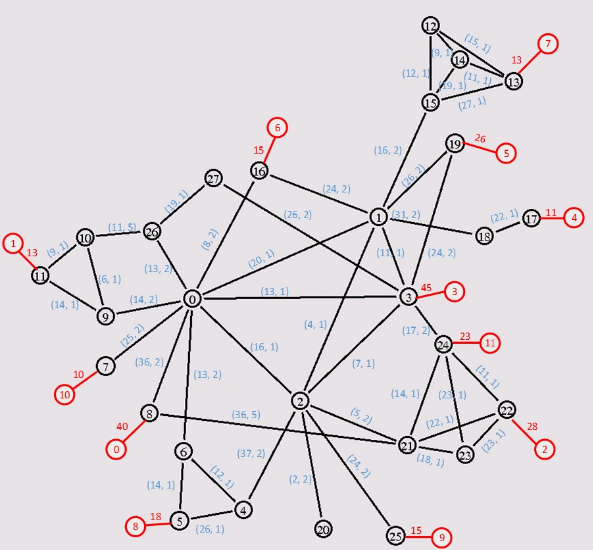
\includegraphics[width=3in]{imgs/网络示例}
	\caption{网络拓扑图示例}
	\label{wlsl}
\end{figurehere}

上图为G省网络拓扑图,黑色圆圈为网络节点,红色圆圈为消费节点,圆圈内的数字为节点编号。节点之间的连线为网络链路。链路上的标记(x, y)中,x表示链路总带宽(单位为Gbps),y表示每Gbps的网络租用费。消费节点相连链路上的数字为消费节点的带宽消耗需求(单位为Gbps)。

现在假设需要在该网络上部署视频内容服务器,满足所有消费节点的需求。一个成本较低的方案如下图所示,其中绿色圆圈表示已部署的视频内容服务器,通往不同消费节点的网络路径用不同颜色标识,并附带了占用带宽的大小:

\begin{figurehere}
	\centering
	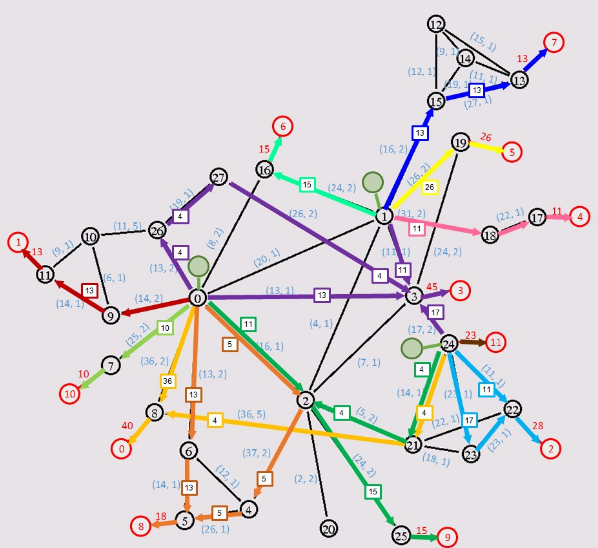
\includegraphics[width=3in]{imgs/方案示例}
	\caption{部署方案示例}
	\label{wlsl}
\end{figurehere}

\section{解决方案}

\subsection{问题分析}

该问题主要分为两个部分,其一,服务器选址,即在网路拓扑图中确定若干网络节点作为服务器节点,用于向消费节点传输视频,和选址问题相似,但有所区别,因为这里和网络流结合而变得更复杂,这也是本问题索要解决的最大难点。第二部分为多源多汇网络流问题,如果第一部分确定了若干网络节点为服务器节点,那么该问题就转化为多源多汇网路流问题,即寻找从若干源点到若干汇点的最小费用的路径,该问题可以通过添加超级源点和超级汇点,转化为最小费用最大流问题。

将该问题的两部分结合来看,该问题实际上是NP问题,即很难寻找到多项式时间内找到该问题的最优解的方法,但是可以在多项式时间内验证一个解是否正确。通常,解决NP问题的方法是启发式算法,启发式算法是相对于最优化算法提出的,在可接受的代价下给出组合优化问题的一个可行解,该可行解与最优解的偏差无法预计,现阶段下的启发式算法主要有蚁群算法、粒子群算法、模拟退火算法、遗传算法,本质上都是玄学算法。

本文同样是采用启发式算法,在分别使用了遗传算法和模拟退火算法之后,效果并不理想(即无法在较少迭代次数下得到较优解),于是尝试将遗传算法和模拟退火算法结合,并得到不错的解。以下介绍算法流程。

\subsection{算法}

\subsection{多源多汇网络流}
\subsubsection{转化}
该问题在确定服务器节点(即源点)之后,就是经典的多源多汇网络流问题,可以直接转化为单源单汇网络流问题,具体操作如下:建立一个(虚拟的)超级源点和一个(虚拟的)超级汇点,将所有源点连接到超级源点,容量和花费分别为无穷大和0,将所有汇点连接到超级汇点,容量和花费分别为消费节点的带宽需求和0。这时,多源多汇网络流问题便转化为最小费用最大流问题,并且由于所有汇点到超级汇点的容量即带宽需求,则最大流只可能小于等于消费节点的带宽总和。

\begin{figurehere}
	\centering
	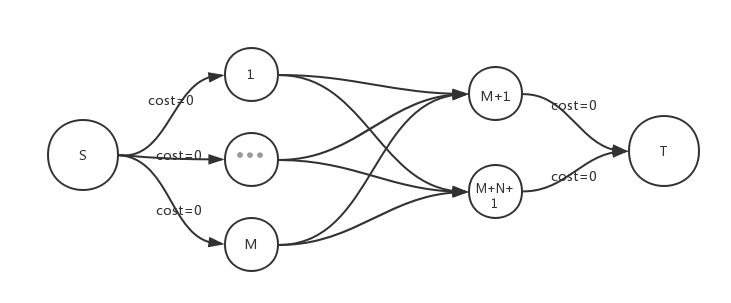
\includegraphics[width=3.4in]{imgs/多源多汇网络流}
	\caption{多源多汇网络流}
	\label{dydhwll}
\end{figurehere}

\subsubsection{最小费用最大流}

在一个网络流中,最大流流量是唯一的,但达到最大流量时是可能有多种路径方案,在这些方案中存在一个最小费用的路径方案。最小费用最大流是网络流中的经典算法,其目的是计算网络流中从源点到汇点达到最大流时能够花费最小费用的路径方案,即$min\{sum(cost(p)*f(p)) | p \in f\}$,其中f为某最大流方案,p是其中的路径,cost(p)是路径p上的代价,f(p)是路径p上的流量。

\paragraph{算法思想}

利用贪心,每次找到一条从源点到汇点的最短路径(路径长度即代价),增加该路径上的流量,直到无法找到一条从源点到达汇点的路径,此时即得到最大流,并且由于每次寻路都是代价最小的路径,因此每次增加的都是最小代价,使得当前最小代价是达到当前流量时的最小代价,因此最后的总代价最小,这里的代价就是指费用。算法步骤如下:

\paragraph{算法步骤}

\begin{enumerate}[(1)]
\item 寻找一条从源点到汇点的最短路径,路径长度即单位带宽费用
\item 计算该条路径上边的最小容量$f$,当前最大流量$max\_flow$扩充$f$,最小费用$min_cost$扩充$f*min\_dist(s,t)$
\item 将这条路径上所有边的正向都减少$f$,反向都增加$f$
\item 重复(1)-(3)知道无法找到从源点到汇点的路径
\end{enumerate}

\subsection{SPFA算法}

本文实现中采用SPFA算法来计算最短路径,SPFA(Shortest Path Faster Algorithm)算法是西安交通大学段凡丁于1994年发表,其在Bellman-ford算法的基础上加上一个队列优化,减少冗余的松弛操作,是一种高效的最短路径算法。

\subsubsection{算法过程}

设立一个队列用来保存待优化的顶点,优化时每次取出队首顶点$u$,并用$u$点当前的最短路径估计值$dist[u]$去松弛与$u$点邻接的顶点$v$。如果$v$点最短路径估计值$dist[v]$比$dist[u]$与$u$、$v$间距离之和$len(u,v)$还要大,则$v$点最短路径值更新为$dist[u]+len(u,v)$,并且如果$v$点不在当前队列中,则将$v$点放入队尾,这样不断从队列中取出顶点进行松弛操作,直至队列空为止。(所谓的松弛操作,简单来说,对于顶点$i$,把$dist[i]$调整更小或更大。)

\subsection{遗传模拟退火算法}

模拟退火算是一种启发式随机搜索算法,它模拟固体物质退火过程的热平衡问题与随机搜索寻优问题的相似性来达到寻找全局最优或近似全局最优的目的。在模拟退火算法的运行过程中融入遗传算法,即模拟退火遗传算法。

在搜索最优解的过程中,模拟退火算法会接收优化解,同时也会随机的、有限度的接受恶化解,并且接收恶化解的概率随着温度的降低会越来越小,前者使得算法可能从局部最优解中跳出到邻域,从而找到更优的解,后者使得算法收敛。

遗传算法是模拟达尔文生物进化论的自然选择和遗传学机理的生物进化过程的计算模型,是一种通过模拟自然进化过程搜索最优解的方法。

\subsubsection{初始状态}

本问题的初始状态,即种群的初始状态。

初始种群由两部分组成,第一部分为服务器节点全部连接到消费节点上。第二部分为随机初始化。种群个体的编码使用二进制形式,i位为0表示该点不设服务器,i位为1表示该点设为服务器,设个体大小(网络节点数目)为N,则总共有$2^N$种可能情况。随机初始化指的是随机选取网络节点为服务器节点。

\subsubsection{遗传模拟退火算法}

\begin{enumerate}
\item 初始化种群大小$geneNum$,交叉概率$P_{cross}$,变异概率$P_{mutation}$,退火速率$r$,增点概率$P_{add}$,退火迭代次数$k=0$
\item 进入模拟退火的迭代阶段,遍历种群中的个体$s_i$,计算费用$f(i)$,在领域中寻找生成新的状态$s_j$,计算费用$f(j)$,接受概率为
$$Accept(s_j)=min(1,exp(-\frac{f(j)-f(i)}{t_k}))$$。若接受则替代原来个体$s_i$作为新个体$s_j$,否则丢弃,用回$s_i$。

这里要分两种情况:
\begin{enumerate}
	\item $f(j)$非-1,即邻域个体有解,若原个体无解,则接受,若原个体有解,则概率性接收。
	\item $f(j)$为-1,即领域个体无解,不接受
\end{enumerate}

若接收,则相应地,个体适应度更新为邻域个体的费用。若不接收,则个体适应度更新为原个体的费用,若为-1(即原个体无解),则用服务器全部放置在消费节点的费用来替代适应度。

\item 遍历种群个体之后,需要计算种群各个体的适应度,计算适应度公式为

$$fitness_i(t_k) = exp(-\frac{f(i)-min\{f\}}{t_k})$$
其中若$f(i)$等于$-1$(即个体非可行解),则用全部服务器放置在消费节点的费用来替代

\item 利用各个体适应度去除以种群总适应度(即个体适应度之和)来得到各个种群的选择概率,然后进行轮盘赌选择、交叉、变异得到下一代种群。再对下一代种群进行从步骤二开始的操作,并更新退火温度$t_{k+1} = t_k * r$。

\end{enumerate}

\section{实验}

选择网络节点数目50、消费节点数目9的5个不同的拓扑网络进行测试,结果分别如下
\begin{tabular}{|c|}
  \hline
  \makecell[cl]{网络结点数: 50, 网络链路数: 96, 消费结点数: 9 \\ 
  每台服务器的费用为: 260 \\ 最小费用:2042 \\ 服务器结点:7, 13, 15, 22, 37, 38, 43} \\
  \hline
  \makecell[cl]{网络结点数: 50, 网络链路数: 97, 消费结点数: 9 \\ 
  每台服务器的费用为: 280 \\ 最小费用:2136 \\ 服务器结点:6, 7, 13, 17, 35, 41, 48} \\
  \hline
  \makecell[cl]{网络结点数: 50, 网络链路数: 113, 消费结点数: 9 \\ 
  每台服务器的费用为: 300 \\ 最小费用:1692 \\ 服务器结点:12, 18, 23, 29, 31, 38, 48} \\
  \hline
  \makecell[cl]{网络结点数: 50, 网络链路数: 97, 消费结点数: 9 \\ 
  每台服务器的费用为: 300 \\ 最小费用:2111 \\ 服务器结点:10, 22, 26, 29, 35} \\
  \hline
  \makecell[cl]{网络结点数: 50, 网络链路数: 99, 消费结点数: 9 \\ 
  每台服务器的费用为: 240 \\ 最小费用:1967 \\ 服务器结点:12, 15, 20, 22, 26, 37, 48} \\
  \hline
\end{tabular}

% \begin{figurehere}
% 	\centering
% 	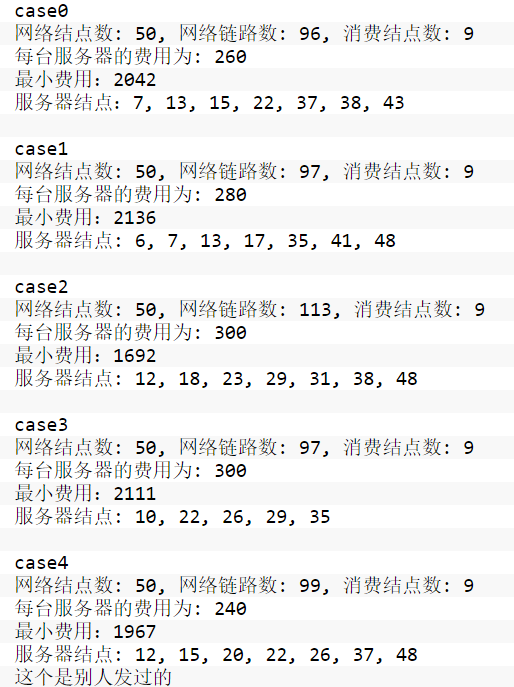
\includegraphics[width=3.4in]{imgs/result}
% 	\caption{结果}
% 	\label{jg}
% \end{figurehere}

上图标注了每个拓扑网络的网络节点数目,消费节点数目,最小费用,服务器节点的选择

\section{结论}

从上述结果看,模拟退火遗传算法得到了不错的结果,比全部服务器放置在消费节点要更优,迭代次数均少于200次,在可以接收的范围以内。

本方法仍然有较多可改进的地方。比如本方法中将初始节点都放置在消费节点上,实际上,可以考虑用贪心的方法进一步改进得到更好的初始节点,另外启发式算法的通病是容易落在局部最优解中,这需要考虑适当的邻域策略跳出局部,从而找到更好的解。另外,本方法中采用SPFA算法寻找路径,可以考虑采用效率更高的ZKW算法缩短每次迭代所需要的时间,以提高方案速率。

%%%%%%%%%%%%%%%%%%%%%%%%%%%%%%%%%%%%%%%%%%%%%%%%%%%%%%%%%%%%%%%%
%  参考文献
%%%%%%%%%%%%%%%%%%%%%%%%%%%%%%%%%%%%%%%%%%%%%%%%%%%%%%%%%%%%%%%%
%\bibliographystyle{IEEEtran}
%\bibliography{IEEEabrv, IEEEexample.bib}


\end{multicols}

\clearpage

\end{document}
